\documentclass[12pt,titlepage,a4page , tikz , multi,table , svgnames,xcdraw]{article}
\usepackage{graphicx}
\usepackage[svgnames , table , xcdraw]{xcolor} 
\usepackage{fancyhdr}
 
\usepackage{hyperref}
\hypersetup{
    colorlinks=true,
    linkcolor=blue,
    filecolor=magenta,      
    urlcolor=cyan,
}
\usepackage{multirow}
\usepackage{graphicx}
\usepackage{float}
\usepackage{enumitem}
\usepackage{listings }
\usepackage[a4paper, total={6in, 8in}]{geometry}
\usepackage{afterpage}
\usepackage{amssymb}
\usepackage{lscape}
\usepackage{amsmath}
\usepackage{svg}
\usepackage[final]{pdfpages}



\usepackage[T1]{fontenc}
\usepackage{tikz}
\usepackage[utf8]{inputenc} % Required for inputting international characters
\usepackage{PTSerif} 

\usepackage{float}

\usepackage{xepersian}
\settextfont[
 BoldFont={XB NiloofarBd.ttf}
 ]{XB Niloofar.ttf}


\NewDocumentCommand{\codeword}{v}{
\texttt{\textcolor{blue}{#1}}
}
\DeclareFixedFont{\ttb}{T1}{txtt}{bx}{n}{12} % for bold
\DeclareFixedFont{\ttm}{T1}{txtt}{m}{n}{12}  % for normal


\definecolor{deepblue}{rgb}{0,0,0.5}
\definecolor{deepred}{rgb}{0.6,0,0}
\definecolor{deepgreen}{rgb}{0,0.5,0}


% Python style for highlighting
\newcommand\pythonstyle{\lstset{
language=Python,
basicstyle=\ttm,
otherkeywords={self},             % Add keywords here
keywordstyle=\ttb\color{deepblue},
emph={MyClass,__init__},          % Custom highlighting
emphstyle=\ttb\color{deepred},    % Custom highlighting style
stringstyle=\color{deepgreen},
frame=tb,                         % Any extra options here
showstringspaces=false            % 
}}


% Python environment
\lstnewenvironment{python}[1][]
{
\pythonstyle
\lstset{#1}
}
{}

% Python for external files
\newcommand\pythonexternal[2][]{{
\pythonstyle
\lstinputlisting[#1]{#2}}}

% Python for inline
\newcommand\pythoninline[1]{{\pythonstyle\lstinline!#1!}}


\begin{document}

\begin{titlepage}

 \begin{center}
        
       \vspace*{1cm}

 \vspace{1cm}
       \textbf{ \Huge{به نام خدا} }
       \vspace{0.4cm}
       
       
\includegraphics[width=0.4\textwidth]{sharif1.png}
       
 	\vspace{0.7cm}
       \textbf{ \LARGE{هوش مصنوعی} }

 
   \vspace{0.7cm}
  \textbf{ \Large{ تمرین پیاده سازی دوم} }
   \vspace{0.5cm}
       
 
      \large \textbf{دانشکده مهندسی کامپیوتر}\\\vspace{0.2cm}
    \large   دانشگاه صنعتی شریف\\\vspace{0.25cm}
      
استاد:\\
    \textbf{{جناب آقای دکتر عبدی}}

    \vspace{0.25cm}
    \noindent\rule[1ex]{\linewidth}{3pt}
    
    \vspace{0.5cm}
نام و نام خانوادگی:\\
    \textbf{{امیرمهدی نامجو}}
        \vspace{0.1cm}

\end{center}
\end{titlepage}

\newpage
\pagestyle{fancy}
\fancyhf{}
\fancyfoot{}

\cfoot{\thepage}
\chead{تمرین پیاده سازی دوم}
\rhead{امیرمهدی نامجو}
\lhead{هوش مصنوعی}




\newpage

\section{کتابخانه‌های موردنیاز}

ابتدا باید این پکیج‌ها برای اجرای درست کد نصب شوند. دستور نصب هر کدام در زیر آمده است:

\begin{latin}
\begin{lstlisting}[language=Python]
pip install numpy
pip install pandas
\end{lstlisting}

\end{latin}

کاربرد این دو که کاملاً مشخص است. تقریباً در هر کاری که مربوط به تحلیل داده باشد، نیاز به استفاده از این دو کتابخانه داریم. در این جا هم کاملاً از DataFrame های pandas استفاده خواهیم کرد.


\begin{latin}
\begin{lstlisting}[language=Python]
pip install scikit-learn
\end{lstlisting}

\end{latin}

از این کتابخانه، صرفاً برای فرآیند تقسیم بندی داده به دو بخش داده تست و آزمایشی استفاده کرده‌ام. از ویژگی‌های دیگر آن نظیر خود پیاده سازی درخت تصمیم، به هیچ وجه استفاده نشده است.


\begin{latin}
\begin{lstlisting}[language=Python]
pip install graphviz
pip install GvGen
\end{lstlisting}

\end{latin}

این دو کتابخانه، برای به تصویر کشیدن گراف به صورت بصری به کار رفته‌اند. باید توجه داشت که graphviz یک موتور رندر گرافیکی گراف است و باید فایل‌های اجرایی آن به صورت جداگانه از سایت آن دانلود و نصب بشوند. همچنین باید اطمینان حاصل کرد که پوشه bin آن در PATH سیستم قرار بگیرد. برای مثال در سیستم‌عامل ویندوز 10 با معماری 64 بیتی، در صورت انتخاب مسیر نصب پیش‌فرض باید این آدرس:
\begin{center}
\begin{latin}
C:\textbackslash Program Files (x86)\textbackslash Graphviz2.38\textbackslash bin
\end{latin}
\end{center}

در PATH سیستم و کاربر قرار بگیرد.

این موتور رندر گرافیکی، در اصل با زبان خاص خودش به نام dot کار می‌کند که زبان قابل فهمی است ولی برای این که خیلی درگیر مراحل تبدیل ساختار درختی ساخته شده توسط خودم به زبان آن نباشم، از کتابخانه GvGen استفاده کرده‌ام. با این کتابخانه به راحتی می‌توان با انجام یک DFS ساده روی ساختار درختی پیاده سازی شده توسط خودم، ارتباطات گراف برای GvGen را تعریف کرده و در نهایت این کتابخانه، کد قابل اجرا توسط graphviz را تولید می‌کند. توجه کنید که اگر یک بار برنامه را اجرا کنید و graphviz خروجی خود را نمایش بدهد، قبل از اجرای مجدد باید خروجی قبلی که یک فایل pdf است، بسته بشود. زیرا graphviz در اجرای بعدی، دوباره اقدام به نوشتن روی همان فایل می‌کند و در صورت باز بودن فایل، با خطا رو به رو خواهد شد.

در صورتی که graphviz را نصب نکرده باشید، می توانید خطوط انتهایی کد را به این شکل تغییر دهید تا به جای نمایش گرافیکی،‌ نمایش متنی گراف را مشاهده کنید:


\begin{latin}
\begin{python}

# makeVisualGraph(mytree)
mytree.display()

\end{python}
\end{latin}


به دلیل همین ایجاد شدن فایل جدید، پروژه باید حتماً در پوشه‌ای اجرا شود که کاربر فعلی دسترسی write روی آن داشته باشد. البته طبیعتاً اگر مثلاً با اکانت adminstrator باشید و یا در لینوکس، فرآیند اجرا از طریق sudo انجام شود، نباید مشکل خاصی پیش بیاید.


\newpage

\section{کد مربوط به بخش رستوران}
ابتدا کد مربوط به این بخش را بر اساس شبه کد اسلایدهای کلاس نوشته‌ام. به ترتیب توابع استفاده شده را در زیر خواهم آورد و کاربرد آن‌ها را توضیح می‌دهم:

\begin{latin}
\begin{python}
def entropy_func(q):
    return -(q * math.log2(q))


def B_func(q):
    if q == 0 or q == 1:
        return 0
    return entropy_func(q) + entropy_func(1 - q)
\end{python}

\end{latin}

تابع اول، صرفاً عبارت پرتکرار استفاده شده در محاسبه آنتروپی را حساب می‌کند و دومی هم بر اساس یک $q$ که بگیرد مقدار $B$ (طبق تعریف اسلایدها) را محاسبه می‌کند. مثلاً $B(0.5)=1$



\begin{latin}
\begin{python}
def remainder(df: pd.DataFrame, col_name, res_name):
    all_p_count = len(df[df[res_name] == 1])
    all_n_count = len(df) - all_p_count;
    all_values = df[col_name].unique()
    s = 0.0
    for k in all_values:
        dcol = df[df[col_name] == k]
        pk = len(dcol[dcol[res_name] == 1])
        nk = len(dcol[dcol[res_name] == 0])
        s = s + ((pk + nk) / (all_p_count + all_n_count)
         * B_func((pk / (pk + nk))))
    return s
\end{python}

\end{latin}

این تابع، طبق تعریف اسلایدها، مقدار remainder را حساب می‌کند. برای این کار هم صرفاً value های موجود در ستون مربوطه DataFrame بررسی می‌شود. زیرا سایر value ها هر چند مقادیر معتبری هم باشند، وقتی در DataFrame نباشند، قطعاً ضریب 0 ایجاد می‌کنند. در متغیرهای ورودی این تابع col\_name مشخص کننده عنوان ستونی (ویژگی) است که قصد تست آن را داریم و \lr{res\_name} هم مشخص کننده نام ستونی است که نتایج در آن نوشته شده‌اند. (برای اینکه برنامه بتواند تعداد موارد مثبت و منفی را بشمارد)

\newpage

\begin{latin}
\begin{python}[language=Python]
def gain(df: pd.DataFrame, col_name, res_name):
    all_p_count = len(df[df[res_name] == 1])
    all_n_count = len(df) - all_p_count;
    entrop = B_func((all_p_count / (all_n_count + all_p_count)))
    rem = remainder(df, col_name, res_name)
    return B_func((all_p_count / (all_n_count + all_p_count)))
     - remainder(df, col_name, res_name), entrop, rem

\end{python}

\end{latin}

این تابع gain را حساب می‌کند و در ضمن، هم gain و هم آنتروپی و هم remaining را بر می‌گرداند که بعداً بتوان در Node ها ذخیره کرد.


\begin{latin}
\begin{python}[language=Python]
def chooseAttribute(df, attributes, res_name):
    attributes_importance = {}
    entropy = {}
    remains = {}
    for attr in attributes:
        attributes_importance[attr], entropy[attr],
         remains[attr] = gain(df, attr, res_name)
    answer = max(attributes_importance.items(),
     key=operator.itemgetter(1))[0]
    return answer, attributes_importance[answer],
     entropy[answer], remains[answer]

\end{python}

\end{latin}

این تابع، نسبت به همه attribute های باقی مانده، میزان gain را بررسی کرده و بر اساس آن بهترین ویژگی را پیدا کرده و به همراه مقادیر مربوط به gain و آنتروپی و remaining آن به تابعی که آن را صدا زده است، return می‌کند.



    
    \begin{latin}
\begin{python}[language=Python]
def isAllSame(df: pd.DataFrame):
    a = df.to_numpy()
    return (a[0] == a[1:]).all()
\end{python}

\end{latin}

این تابع بررسی می‌کند که آیا تمامی اعضای یک DataFrame یکی هستند یا نه. در اصل در هنگام کاربرد، فقط یک ستون DataFrame را که شامل نتایج است به آن پاس می‌دهیم که صرفاً ببیند که آیا به تقسیم بندی رسیده‌ایم که همه در آن یکسان باشند یا نه.

\newpage



    \begin{latin}
\begin{python}[language=Python]
class DecisionFork:
    def __init__(self, attr, default_child=None, branches=None,
     entropy=None,gain_=None, remainder_=None):
        self.attr = attr
        self.default_child = default_child
        self.branches = branches or {}
        self.entropy = entropy
        self.gain_ = gain_
        self.remainder_ = remainder_

    def __call__(self, example):

        attr_val = example[self.attr]
        if attr_val in self.branches:
            return self.branches[attr_val](example)
        else:

            return self.default_child(example)

    def add(self, val, subtree):

        self.branches[val] = subtree

    def display(self, indent=0):
        name = self.attr
        print('Test', name)
        for (val, subtree) in self.branches.items():
            print(' ' * 4 * indent, name, '=', val, '==>',
             end=' ')
            subtree.display(indent + 1)

    def __str__(self):
        return str(self.attr + '\n' + 'Entropy =' + str(self.entropy)
         + '\n' + 'Gain =' +
                   str(self.gain_) + '\n' +
                    'Remainder =' + str(self.remainder_))
\end{python}

\end{latin}

این کلاس مربوط به پیاده سازی Node های تصمیم گیری می‌شود. عناصر اصلی آن یکی attr است که نام attribute مورد تست را ذخیره می‌کند. دیگری defualt\_child است که در اصل برای هر گره این را قرار می‌دهیم که در صورتی که در میان مواردی که در داده‌اموزشی داریم، مقدار خاصی موجود نبود  و در مورد آن مقدار train صورت نگرفت، در صورتی که در تست به آن برخورد کرد، سراغ کدام حالت برود. branches که یک آرایه است که همه Node های فرزند این Node را نگه می‌دارد. سه مورد بعدی هم که اطلاعات مربوط به آنتروپی و ... این گره هستند.

تابع \_\_call\_\_ هم برای این است که بتوانیم خود این Node را مانند یک تابع روی یک مثال صدا بزنیم و به صورت بازگشتی، مراحل مختلف تا رسیدن به نتیجه طی شود.

تابع display هم در ابتدا برای نمایش متنی درخت به صورت بازگشتی و با indentation متفاوت برای فرزندان، طوری که ساختار درختی مشخص شود، قرار داده بودم که اکنون که بعداً که امکان رسم گرافیکی را فراهم کردم، عملاً این تابع کارایی ندارد.


\begin{latin}
\begin{python}[language=Python]
class DecisionLeaf:

    def __init__(self, result, entropy=None):
        self.result = result
        self.entropy = entropy

    def __call__(self, example):
        return self.result

    def display(self, indent=0):
        print('RESULT =', self.result)

    def __str__(self):
        return ' ' + str(self.result) + '\n' +
         'Entropy =' + str(self.entropy)

\end{python}

\end{latin}

این کلاس هم همان طور که مشخص است، برای نقاط برگ که نتیجه نهایی مشخص می‌شود، مورد استفاده قرار گرفته است.



    \begin{latin}
\begin{python}[language=Python]
def pluarlity_value_node(df: pd.DataFrame, outcome_name):
    all_p_count = len(df[df[outcome_name] == 1])
    all_n_count = len(df) - all_p_count;
    entropy = B_func((all_p_count / (all_n_count + all_p_count)))

    return DecisionLeaf(df.mode()[outcome_name][0], entropy=entropy)


\end{python}

\end{latin}

این تابع برای ساخت یک DecisionLeaf استفاده می‌شود. به این شکل که بررسی می‌کند فراوانی کدام یک از موارد Outcome در DataFrame داده شده بیش‌تر است و آن را به عنوان نتیجه DecisionLeaf انتخاب می‌کند. ضمناً entropy را هم حساب کرده و در DecisionLeaf قرار می‌دهد.

\newpage


   \begin{latin}
\begin{python}[language=Python]

def DecisionTreeLearning(examples: pd.DataFrame, attributes: list,
 parent_examples, outcome_name, curr_depth, max_depth=6):
    if examples.empty:
        return pluarlity_value_node(parent_examples, outcome_name)
    if isAllSame(examples[outcome_name]):
        return DecisionLeaf(examples[outcome_name].iloc[0], entropy=0)
    if not attributes:
        return pluarlity_value_node(examples, outcome_name)
    if curr_depth == max_depth:
        return pluarlity_value_node(examples, outcome_name)
    cols = list(examples.columns)
    cols.remove('Outcome')
    attr, gain_, entropy_, remains_ = chooseAttribute(examples, cols,
     outcome_name)
    all_values = examples[attr].unique()
    tree = DecisionFork(attr,
     pluarlity_value_node(examples, outcome_name),
     gain_=gain_, entropy=entropy_,remainder_=remains_)
    for vk in all_values:
        new_cols = attributes
        if (attr in new_cols):
            new_cols.remove(attr)
        subtree = DecisionTreeLearning(examples[examples[attr] == vk],
         new_cols, examples, outcome_name, curr_depth + 1, max_depth)
        tree.add(vk, subtree)
    return tree
\end{python}

\end{latin}

این تابع اصلی اجرای الگوریتم است که مطابق با سودوکدی که در اسلایدهای درس بوده، پیاده سازی شده است. صرفاً یکسری تفاوت‌های کوچک نظیر ذخیره سازی مقادیر آنتروپی و... دارد که در عملکرد نهایی تأثیری ندارند و صرفاً باعث ذخیره اطلاعات بیش‌تری در هر Node می‌شود که در آینده برای نمایش آن‌ها از آن استفاده می‌کنیم.

تنها تفاوت قابل تمایز در خود الگوریتم این است که در این جا من max\_depth هم تعیین کرده‌ام که عمق درخت از یک حدی بیش‌تر نشود و اگر خواست از آن عمق بیش‌تر بشود، بر اساس مقادیر فعلی، یک گره برگ در آن نقطه قرار خواهد گرفت.

\newpage


   \begin{latin}
\begin{python}[language=Python]

def graphMaker(g, mytree):
    if isinstance(mytree, DecisionLeaf):
        myItem = g.newItem(mytree.__str__())
        return myItem
    elif isinstance(mytree, DecisionFork):
        myItem = g.newItem(mytree.__str__())
        for key, val in mytree.branches.items():
            newTree = graphMaker(g, val)
            l = g.newLink(myItem, newTree)
            g.propertyAppend(l, "color", "blue")
            g.propertyAppend(l, "label", key)
        return myItem


def makeVisualGraph(mytree):
    g = gvgen.GvGen()
    graphMaker(g, mytree)
    string = ""
    myfile = open("output_graphviz.txt", 'w')

    g.dot(myfile)
    myfile.close()
    myfile = open("output_graphviz.txt", 'r')
    lines = myfile.readlines()[1:]
    for line in lines:
        string = string + line

    srcc = Source(string)
    srcc.render(view=True)

\end{python}

\end{latin}

این دو تابع برای رسم گراف با کمک graphviz و GvGen به کار رفته‌اند. تنها نکته قابل توجه این است که GvGen خروجی که تولید می‌کند، الزاماً وارد یک فایل text می‌شود و در نتیجه باید ابتدا فایل text ذخیره شود، سپس دوباره اطلاعات از آن خوانده شده، در قالب یک string در آمده و توسط کلاس Source که در کتابخانه graphviz تعریف شده است، این string رندر بشود.

\newpage


   \begin{latin}
\begin{python}[language=Python]

df = pd.read_csv('restaurant.csv')

cols = list(df.columns)
cols.remove('Outcome')

mytree = DecisionTreeLearning(df, cols, None, 'Outcome', 0, 6)
makeVisualGraph(mytree)

\end{python}

\end{latin}

در نهایت این چند خط هم برای اجرای کد روی restaurant.csv که در فایل فشرده‌ای که ارسال کرده‌ام، قرار دارند، قرار گرفته است. این فایل را خودم ساختم و در آن برای بیان کردن داده‌های رشته‌ای سؤال نظیر Full و... نماد گذاری عددی به این شکل استفاده کرده‌ام:

\begin{latin}

Pat: None: 0

Pat: Some: 1

Pat: Full: 2

Type: French: 0

Type: Thai: 1

Type: Burger: 2

Type: Italian: 3

Est: 0-10 : 0

Est: 10-30: 1

Est: 30-60: 2

Est: >60: 3


\end{latin}

نتیجه نهایی در صفحه بعد قرار دارد:

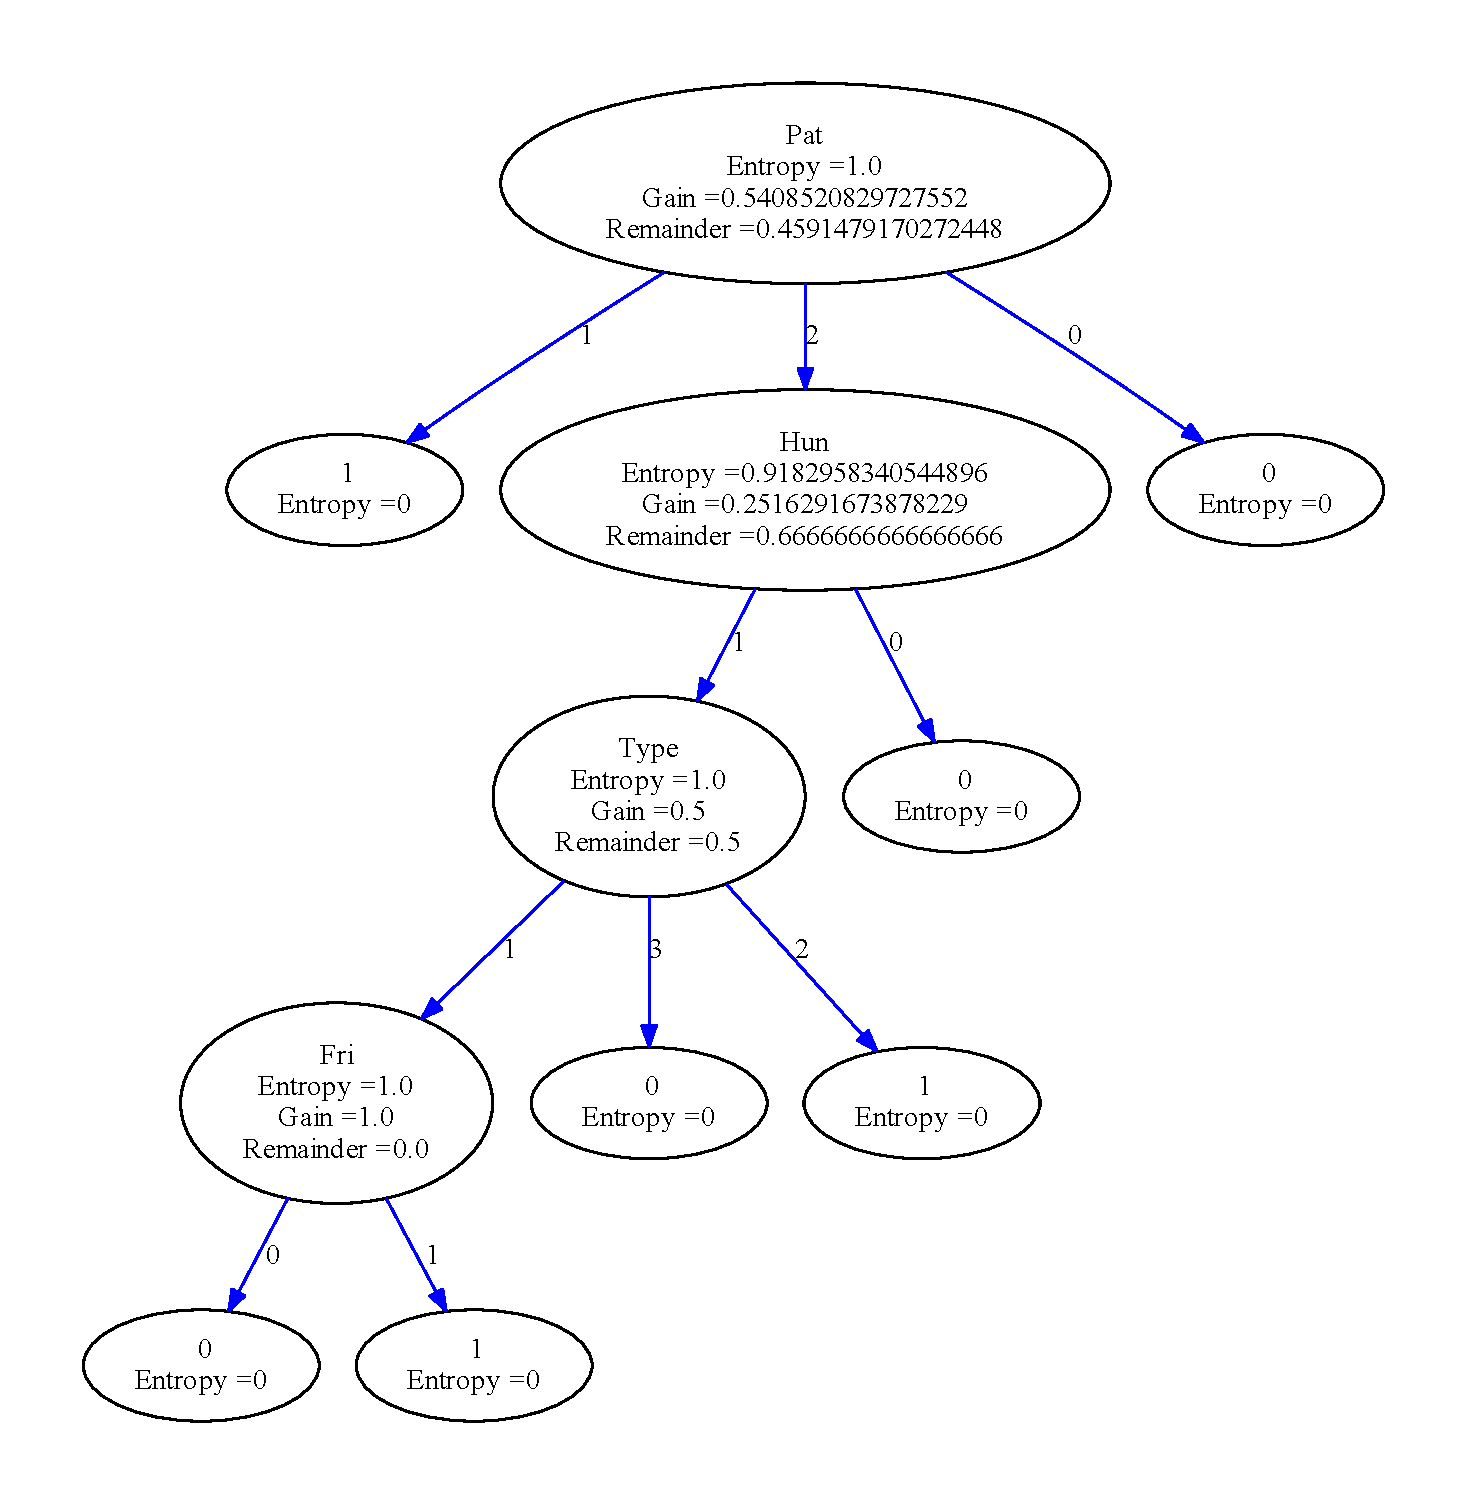
\includepdf[pages=-,pagecommand={},width=\textwidth]{DecTree.pdf}

همان طور که واضح است، این نتیجه مطابق با شکلی است که در اسلایدها قرار گرفته است. زیرا عیناً همان الگوریتم پیاده سازی شده است و صرفاً ویژگی اضافه max\_depth را من به الگوریتم اضافه کردم اما همچنان چون آن را به اندازه کافی (6) بزرگ داده‌ام، نتیجه نهایی همین به دست آمده است.

\newpage

\section{کد مربوط به بخش دیابت}

ابتدا، کدهایی Preprocess کردن داده‌ها را توضیح می‌دهم.


   \begin{latin}
\begin{python}[language=Python]

def discrete_find_bins(df: pd.DataFrame, column_name, number_of_bins):
    maxi = df[column_name].max()
    mini = df[column_name].min();
    diff = (maxi - mini) / number_of_bins
    bins = []
    bins.append(round(mini - diff, 2))
    for i in range(number_of_bins):
        bins.append(round(mini + diff * i, 2))
    bins.append(round(maxi, 2))
    bins.append(round(maxi + diff, 2))
    return bins
\end{python}

\end{latin}

این تابع، بر اساس دیتافریمی که به آن داده می‌شود و نام ستونی که داده شده است و تعداد دسته‌هایی که می‌خواهیم را وارد می‌کنیم و این تابع مرزهای دسته‌ها را ساخته و در قالب یک لیست بر می‌گرداند. برای یک بازه کمتر از minimum و یک بازه بیش‌تر از maximum هم یک بازه در نظر گرفته می‌شود.

  \begin{latin}
\begin{python}[language=Python]


def discrete_column(df: pd.DataFrame, column_name, bins_):
    label = []
    for i in range(len(bins_) - 1):
        label.append(i)
    dfnew = df.copy()
    dfnew[column_name + '-binned'] = pd.cut(x=df[column_name],
     bins=bins_, labels=label)
    return dfnew

\end{python}

\end{latin}

این تابع، داده‌های یک ستون را بر اساس bin ای که به آن داده می‌شود، گسسته سازی می‌کند. برای عملیات گسسته سازی، از تابع cut در کتابخانه pandas استفاده شده است. این داده‌ها در یک دیتافریم جدید قرار می‌گیرند که یک ستون اضافی دارد که به نام آن، کلمه binned اضافه شده است. مثلاً اگر نام ستون اولیه Glucose بوده باشد، نام ستون جدید Glucose-binned خواهد بود.

\newpage


  \begin{latin}
\begin{python}[language=Python]



def preprocess(train: pd.DataFrame, test: pd.DataFrame):
    col_name = list(train.columns)
    Pregnancies_bins = discrete_find_bins(train, 'Pregnancies', 5)
    Glucose_bins = discrete_find_bins(train, 'Glucose', 5)
    BloodPressure_bins = discrete_find_bins(train, 'BloodPressure', 5)
    SkinThickness_bins = discrete_find_bins(train, 'SkinThickness', 5)
    Insulin_bins = discrete_find_bins(train, 'Insulin', 5)
    BMI_bins = discrete_find_bins(train, 'BMI', 5)
    DiabetesPedigreeFunction_bins = discrete_find_bins(df,
     'DiabetesPedigreeFunction', 5)
    Age_bins = discrete_find_bins(df, 'Age', 5)

    train = discrete_column(train, 'Pregnancies', Pregnancies_bins)
    train = discrete_column(train, 'Glucose', Glucose_bins)
    train = discrete_column(train, 'BloodPressure', BloodPressure_bins)
    train = discrete_column(train, 'SkinThickness', SkinThickness_bins)
    train = discrete_column(train, 'Insulin', Insulin_bins)
    train = discrete_column(train, 'BMI', BMI_bins)
    train = discrete_column(train,
     'DiabetesPedigreeFunction', DiabetesPedigreeFunction_bins)
    train = discrete_column(train, 'Age', Age_bins)

    test = discrete_column(test, 'Pregnancies', Pregnancies_bins)
    test = discrete_column(test, 'Glucose', Glucose_bins)
    test = discrete_column(test, 'BloodPressure', BloodPressure_bins)
    test = discrete_column(test, 'SkinThickness', SkinThickness_bins)
    test = discrete_column(test, 'Insulin', Insulin_bins)
    test = discrete_column(test, 'BMI', BMI_bins)
    test = discrete_column(test,
     'DiabetesPedigreeFunction', DiabetesPedigreeFunction_bins)
    test = discrete_column(test, 'Age', Age_bins)

    col_name.remove('Outcome')

    return train.drop(col_name, axis=1), test.drop(col_name, axis=1)


\end{python}

\end{latin}

این تابع گسسته سازی ستون‌های کل داده‌ها را انجام می‌دهد. دسته‌بندی‌های گسسته سازی آن بر اساس داده train ساخته می‌شود و سپس داده‌های train و test بر اساس آن گسسته سازی می‌شوند و ستون‌های قبلی آنان که گسسته نیست هم حذف می‌شود که در اجرای الگوریتم مشکل ایجاد نشود. البته توجه کنید که این توابع یک کپی از DataFrame اصلی تهیه می‌کنند و DataFrame اصلی را خراب نمی‌کنند. دسته‌بندی همه بخش‌ها را هم 5 تایی انجام دادم. زیرا با بررسی‌هایی که کردم، این حالت نتیجه نسبتاً خوبی (تقریباً برابر با نتیجه‌ای که با اجرای توابع آماده کتابخانه sklearn به دست می‌آید) به ما خواهد داد.


\begin{latin}
\begin{python}
def correction_test(test, mytree):
    right_guess = 0

    for i in range(len(test)):
        test_res = mytree(test.iloc[i])
        if test_res == test.iloc[i].Outcome:
            right_guess += 1

    return (right_guess / len(test) * 100)

\end{python}


\end{latin}


این تابع هم صحت الگوریتم را می‌سنجد. می‌توان این تابع را هم بر روی داده train و هم بر روی test اجرا کرد.

ابتدا کد را نسبت به الگوریتم قبلی تست کردم. بخش اجرا کننده و تست کننده داده‌ها به این شکل است:

  \begin{latin}
\begin{python}[language=Python]


df = pd.read_csv('diabetes.csv')
train, test = train_test_split(df, test_size=0.5)
train, test = preprocess(train, test)

cols = list(df.columns)
cols.remove('Outcome')

mytree = DecisionTreeLearning(train, cols, None, 'Outcome', 0, 6)

makeVisualGraph(mytree)

right_guess = 0
for i in range(len(test)):
    test_res = mytree(test.iloc[i])
    if test_res == test.iloc[i].Outcome:
        right_guess += 1

print(right_guess)
print(len(test))
print(right_guess / len(test) * 100)

\end{python}

\end{latin}


در ابتدا، با استفاده از تابع آماده کتابخانه sickit-learn تقسیم بندی داده به دو بخش train و test را انجام دادم. سپس کد را اجرا کرده و درخت را ساختم و پس از آن، روی کل داده‌های تست، درخت را تست کردم و تعداد نتایج درست را شمردم. با چند بار اجرا، دقت‌هایی بین 65 تا 72 درصد را دریافت کردم. دقت داده‌های train هم حدود 86 درصد به دست آمد که نشان می‌دهد تا حدی overfit پیش‌آمده است اما آن‌قدر شدید نیست.

شکل تولید شده توسط آن بسیار بزرگ است و تنها فایل آن را در کنار فایل‌های ارسالی قرار داده‌ام. توصیه می‌شود این فایل را با نرم افزار \lr{Foxit Phantom PDF} باز کنید. چون ظاهراً \lr{Adobe Reader} محدودیت عرض صفحه PDF دارد و نمی‌تواند آن را به درستی نمایش بدهد.

\newpage

یک کد دیگر هم نوشتم که تا حد زیادی شبیه الگوریتم قبلی است. با این تفاوت که این بار به ازای تمامی مقادیر شاخه نمی‌سازیم. بلکه تقسیم‌بندی‌ها به صورت دو شاخه‌ای و بسته به این که مقادیر از یک عددی بزرگ‌تر هستند یا کوچک‌تر صورت خواهد گرفت. برای انتخاب مقدار و attribute مناسب هم بین همه آن‌ها بررسی می‌شود. توجه داریم که به خاطر گسسته سازی، مقادیر مورد بررسی آن‌قدر زیاد نخواهند بود و می‌توان همه را بررسی کرد.

ضمناً به شکل عجیبی، بعضاً شاهد بودم که الگوریتم با وجود این که مقادیر همه یکسان شده بودند، همچنان در حال تکرار یک شرط بود، در نتیجه مجبور شدم یک شرط دیگر هم بگذارم که اگر entropy از $10^{-15}$ کم‌تر بود، باز هم حالت یکسان شدن داده‌ها بگیرد و آن نقطه را برگ بسازد.

در ادامه کدهای بخش‌های مختلف این کد که تا حدی زیادی شبیه قسمت قبل است و صرفاً در بخش‌هایی، متناسب با این که در این جا صرفاً بر اساس کوچک‌تر یا بزرگ‌تر بودن نسبت به یک داده تصمیم گیری می‌کنیم و نه همه داده‌ها، تغییراتی در آن رخ داده است.

در زمینه آنتروپی هم این طور شده است که در اصل، ما با نوعی در هر مرحله، بر اساس موردی که می‌خواهیم داده‌ها را بر اساس آن بشکنیم، به دو دسته می‌رسیم. روش محاسبه Gain من به این شکل بوده که ابتدا برای هر کدام از دو دسته، مقدار آنتروپی را به طور جداگانه حساب کرده‌ام. که مثلاً $e_1$ و $e_2$ به دست می‌آید. سپس بر اساس این که مثلاً یک دسته تعداد داده‌های بیش‌تری دارد و یکی $n_1$ و دیگری $n_2$ داده دارد، به شکل
$Remain =\frac{n_1}{n_1 + n_2} \times e1 + \frac{n_2}{n_1 + n_2} \times e2$
حساب کرده‌ام و در نهایت، بر اساس این که در ابتدا مثلاً $p$ داده مثبت و $q$ داده منفی داشته‌ایم، Gain را به صورت:
$B(\frac{p}{p+q}) - Remain$
حساب کرده‌ام.

در ادامه و از صفحه بعد فقط بخش‌هایی از کد که نسبت به قبل دچار تغییر شده‌اند را نوشته‌ام:

\newpage

  \begin{latin}
\begin{python}[language=Python]


def entropy_of_div(divDf, output_name):
    pk = len(divDf[divDf[output_name] == 1])
    nk = len(divDf[divDf[output_name] == 0])
    if (pk + nk == 0):
        return 0
    return B_func((pk / (pk + nk)))


def entropy_of_all_div(df, col_name, res_name, cutoff):
    leftDf = df[df[col_name] < cutoff]
    rightDf = df[df[col_name] >= cutoff]
    left_entropy = entropy_of_div(leftDf, res_name)
    right_entropy = entropy_of_div(rightDf, res_name)
    entropy_total = (len(leftDf) / len(df) * left_entropy)
     + (len(rightDf) / len(df) * right_entropy)
    return entropy_total


def gain(df, col_name, res_name, cutoff):
    all_p_count = len(df[df[res_name] == 1])
    all_n_count = len(df[df[res_name] == 0])
    current_entropy = B_func(all_p_count / (all_p_count + all_n_count))
    remainder = entropy_of_all_div(df, col_name, res_name, cutoff)
    gain_ = current_entropy - remainder
    return gain_, current_entropy, remainder

\end{python}

\end{latin}

این توابع متناسب با فرمولی که در بالا گفتم، آنتروپی و gain را حساب می‌کند. تابع entropy\_of\_div وظیفه محاسبه آنتروپی یک قسمت تقسیم شده را دارد و تابع دوم، آنتروپی کل (با جمع وزن دار) را بر اساس هر دو قسمت تقسیم (به قسمت کوچک‌تر از مقدار \lr{cutoff} و بزرگ‌تر از \lr{cutoff}) محاسبه می‌کند.

\newpage

 \begin{latin}
\begin{python}[language=Python]


class DecisionFork:
    def __init__(self, attr, cutoff, default_child=None, entropy=None,
     gain_=None, remainder_=None):
        self.attr = attr
        self.cutoff = cutoff
        self.default_child = default_child
        self.left_node = None
        self.right_node = None
        self.entropy = entropy
        self.gain_ = gain_
        self.remainder_ = remainder_

    def __call__(self, example):

        attr_val = example[self.attr]
        if attr_val < self.cutoff:
            return self.left_node(example)
        else:
            return self.right_node(example)

    def add(self, subtree, isLeft):

        if (isLeft):
            self.left_node = subtree
        else:
            self.right_node = subtree

    def display(self, indent=0):
        name = self.attr
        print('Test', name)
        print(' ' * 4 * indent, name, '<', self.cutoff, '==>', end=' ')
        self.left_node.display(indent + 1)
        print(' ' * 4 * indent, name, '>=', self.cutoff, '==>', end=' ')
        self.right_node.display(indent + 1)

    def __str__(self):
        return str(self.attr + '\n' + str(self.cutoff)
         + '\n' + 'Entropy =' + str(self.entropy) + '\n' + 'Gain =' +
                   str(self.gain_) + '\n' + 'Remainder ='
                    + str(self.remainder_))

\end{python}

\end{latin}

تغییر کوچکی در این بخش کد داریم که به جای ذخیره سازی تعداد زیادی از branch های مختلف، به دلیل این که تقسیم‌بندی‌ها دو تایی (مقادیر کمتر از \lr{cutoff} و بیش‌تر مساوی \lr{cutoff}) خواهد بود، تنها Node سمت چپ و راست داریم. ضمن این که مقدار cutoff های باید ذخیره شود و در تابع \_\_call\_\_ هم تغییراتی متناسب با نحوه اعمال متفاوت این درخت تصمیم داریم.


 \begin{latin}
\begin{python}[language=Python]


def chooseAttribute(df: pd.DataFrame, attributes, res_name):
    attributes_importance = {}
    entropy = {}
    remains = {}
    for att in attributes:
        possible_values = df[att].unique()
        for val in possible_values:
            index = (att, val)
            attributes_importance[index], entropy[index], remains[index]
             = gain(df, att, res_name, val)
    answer = max(attributes_importance.items(),
     key=operator.itemgetter(1))[0]
    return answer, attributes_importance[answer], entropy[answer],
     remains[answer]


\end{python}

\end{latin}

این تابع تغییر یافته هم برای انتخاب attribute و مقدار مناسب برای cutoff است که همه حالات را بررسی می‌کند و به عنوان خروجی، هم attribute هم مقدار cutoff و هم آنتروپی و هم reamin و هم Gain را (با عنوان \lr{attributes\_importance}) به تابعی که آن را فراخوانده است، باز می‌گرداند.

\newpage


 \begin{latin}
\begin{python}[language=Python]


def DecisionTreeLearning(examples: pd.DataFrame,
 attributes: list, parent_examples, outcome_name, curr_depth,
                         max_depth=6):
    if examples.empty:
        return pluarlity_value_node(parent_examples, outcome_name)
    if isAllSame(examples[outcome_name]):
        return DecisionLeaf(examples[outcome_name].iloc[0], entropy=0)
    if not attributes:
        return pluarlity_value_node(examples, outcome_name)
    if curr_depth == max_depth:
        return pluarlity_value_node(examples, outcome_name)
    cols = list(examples.columns)
    cols.remove(outcome_name)
    attr, gain_, entropy_, remains_ =
     chooseAttribute(examples, cols, outcome_name)
    if (entropy_ < 1e-15):
        return DecisionLeaf(examples[outcome_name].iloc[0], entropy=0)
    tree = DecisionFork(attr[0], attr[1],
     pluarlity_value_node(examples, outcome_name), gain_=gain_, entropy=entropy_,
                        remainder_=remains_)
    new_cols = attributes

    subtree_left = DecisionTreeLearning(examples[examples[attr[0]] < attr[1]],
     new_cols, examples, outcome_name,
                                        curr_depth + 1,
                                        max_depth)
    tree.add(subtree_left, True)
    subtree_right = DecisionTreeLearning(
    examples[examples[attr[0]] >= attr[1]],
     new_cols, examples, outcome_name,curr_depth + 1,max_depth)
    tree.add(subtree_right, False)
    return tree

\end{python}

\end{latin}

نکته مهم این است که در این جا دیگر روی همه مقادیر، branch و subtree ایجاد نمی‌کنیم و صرفاً یک زیردرخت راست و یک زیردرخت چپ ایجاد می‌کنیم. الگوریتم ایجاد کردن هم در هر دو روش ما، به صورت Depth-First بوده است.

ضمناً در این جا یک شرط

\begin{latin}
\begin{python}[language=Python]

    if (entropy_ < 1e-15):
        return DecisionLeaf(examples[outcome_name].iloc[0], entropy=0)
\end{python}

\end{latin} 

هم اضافه کرده‌ام. زیرا به طرز عجیبی، گاهی اوقات با وجود این که همه یکسان شده بودند، الگوریتم بالا به درستی تشخیص نمی‌داد ولی وقتی شرط را بر اساس آنتروپی تعریف کردم، مشکل برطرف شد.


در نهایت تغییرات کوچکی هم در توابع سازنده نمایش گرافیکی این درخت ایجاد شد به دلیل تغییر ساختار از حالت چند شاخه به حالت دو شاخه:



\begin{latin}
\begin{python}[language=Python]

   def graphMaker(g, mytree):
    if isinstance(mytree, DecisionLeaf):
        myItem = g.newItem(mytree.__str__())
        return myItem
    elif isinstance(mytree, DecisionFork):
        myItem = g.newItem(mytree.__str__())

        left_tree = graphMaker(g, mytree.left_node)
        l = g.newLink(myItem, left_tree)
        g.propertyAppend(l, "color", "blue")
        g.propertyAppend(l, "label", '<')
        right_tree = graphMaker(g, mytree.right_node)
        l2 = g.newLink(myItem, right_tree)
        g.propertyAppend(l2, "color", "blue")
        g.propertyAppend(l2, "label", '>=')
    return myItem


def makeVisualGraph(mytree):
    g = gvgen.GvGen()
    graphMaker(g, mytree)
    string = ""
    myfile = open("output_graphviz.txt", 'w')

    g.dot(myfile)
    myfile.close()
    myfile = open("output_graphviz.txt", 'r')
    lines = myfile.readlines()[1:]
    for line in lines:
        string = string + line

    srcc = Source(string)
    srcc.render(view=True)
\end{python}

\end{latin} 


کد تست کننده مدار هم این است:

\begin{latin}

\begin{python}

df = pd.read_csv('diabetes.csv')
train, test = train_test_split(df, test_size=0.5)
train, test = preprocess(train, test)

cols = list(df.columns)
cols.remove('Outcome')

mytree = DecisionTreeLearning(train, cols, None, 'Outcome', 0, 10)
#
#
makeVisualGraph(mytree)

print(correction_test(test,mytree))

print(correction_test(train,mytree))

\end{python}
\end{latin}

با این الگوریتم، با چند بار اجرا به دقت حدود 65 تا 75 درصد دست یافتم. اکثر اوقات حدود 70 درصد. در حالتی که با عمق 10 اجرا کردم، دقت داده train حدود 95 درصد شد که نشان از overfit بالا دارد. وقتی عمق را به 6 کاهش دادم، دقت داده train حدود 78 و دقت داده تست همان 70 درصد ماند. این نشان می‌دهد که ظاهراً خیلی نمی‌توان با الگوریتم فعلی، وضعیت نتیجه‌ای که از داده تست می‌گیریم را بهبود بخشید.

شکل دو تا از درخت‌های به دست آمده آن را در صفحه بعد قرار داده‌ام. دلیل تفاوت نتایج در هر دفعه این است که در هر بار، داده‌های متفاوتی برای train و تست انتخاب می‌شوند. فایل آن هم در کنار فایل‌های ارسالی قرار دارد. یکی با عمق 10 و دیگری با عمق 6 است. (عمق هم تا قبل از ایجاد برگ‌ها محاسبه شده است)

توجه کنید امکان زوم کردن روی شکل تا هر حدی که بخواهید وجود دارد.

\newpage


\includepdf[pages=-,pagecommand={},width=\textwidth]{DecTree3.pdf}


\newpage


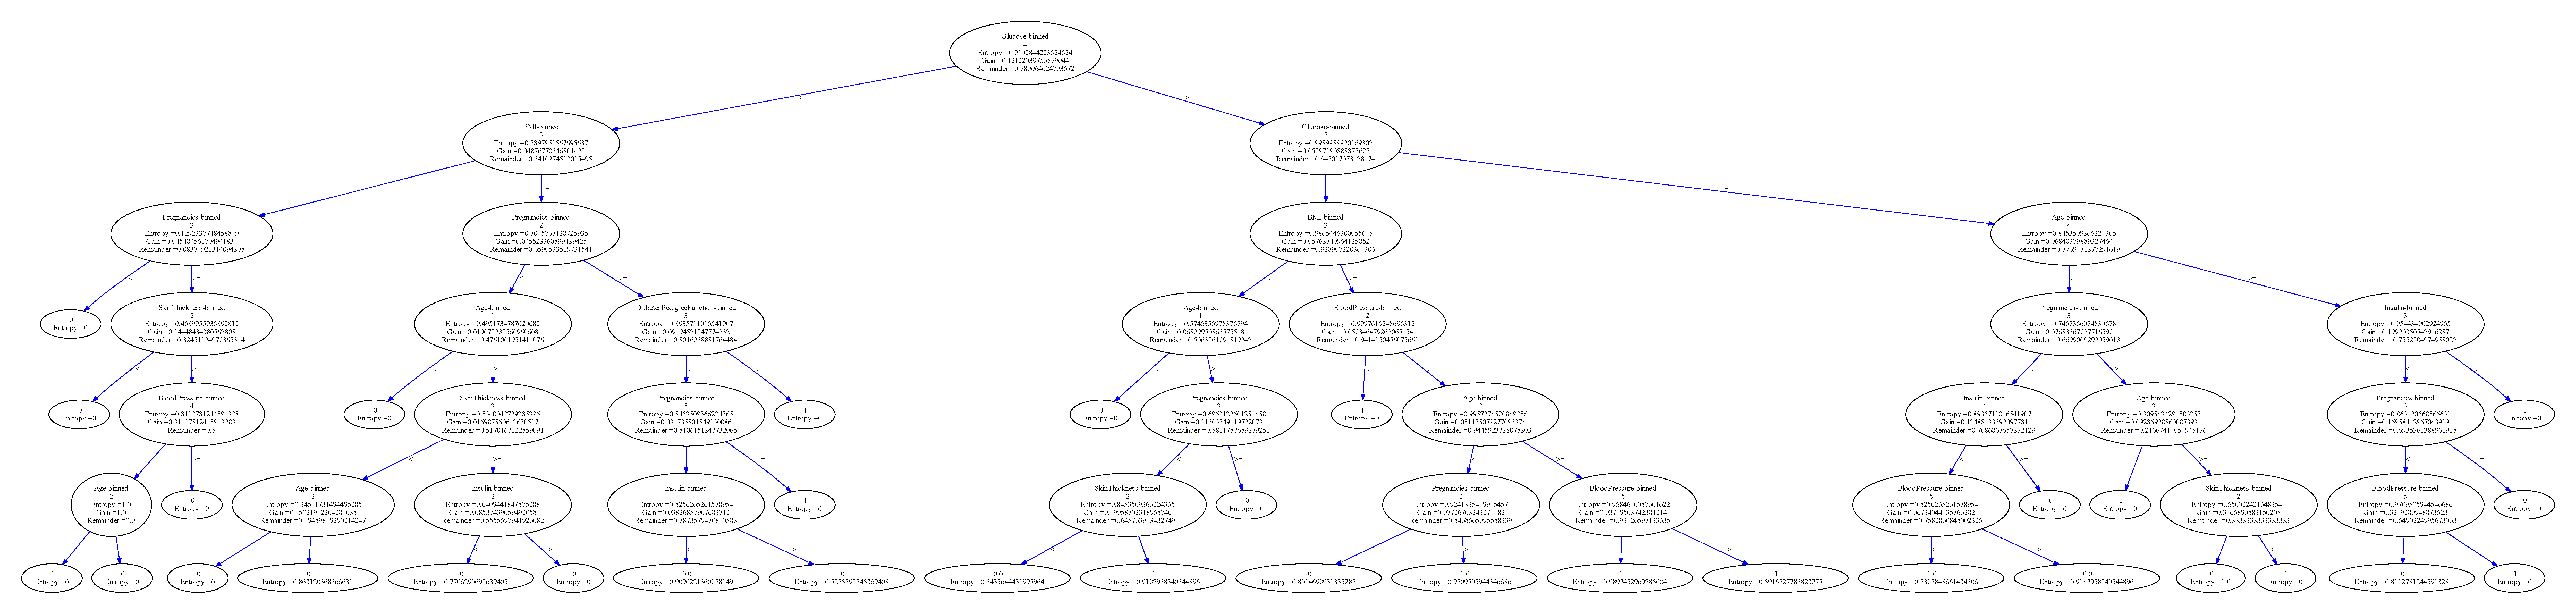
\includepdf[pages=-,pagecommand={},width=\textwidth]{DecTree4.pdf}

\newpage

\section{نتایج}

در نهایت، با کارهایی که انجام دادم و حتی تست کردن این داده‌ها با کتابخانه آماده sickit-learn و رسیدن به دقت حدود 70 درصد در آن، به این نتیجه رسیدم که احتمالاً با روش‌های معمول و حتی کمی بهبود یافته تر از چیزی که نوشته‌ام، نمی‌توان خیلی دقت را در زمینه این داده‌ها افزایش داد. اصلی‌ترین مشکل هم این است که فایل csv داده شده، داده‌های پرت زیادی دارد. نظیر فشار خون $0$، شاخص BMI برابر $0$ و چنین مواردی که در افراد زیادی بروز کرده‌اند. تعداد نسبتاً قابل توجه این موارد، باعث می‌شود که کیفیت کلی کار را نتوان از حد مشخصی بالاتر برد. از این رو بهترین ایده‌ای که برای افزایش دقت به نظرم می‌رسد (و البته عملی نکرده‌ام) این است که خود داده‌ها را تا حدی مرتب‌تر بکنیم و مثلاً برای یکسری از داده‌های پرت، میانگین سایر داده‌ها را قرار بدهیم تا شاید بتوانیم عملکرد بهتری بگیریم. همچنین شاید پیاده سازی ایده هرس کردن هم تا حدی (اما نه خیلی زیاد) بتواند کمک بکند. اما با توجه به این که می‌بینیم کتابخانه‌های آماده‌ای که مدت زیادی روی آن‌ها کار شده است هم همچنان دقتی در حدود الگوریتم من می‌دهند، نشان می‌دهد که با روش‌های معمول و از روی خود این داده‌ها، نمی‌توان خیلی دقت را بالاتر برد.

در مورد بیش برازش، در زمانی که عمق درخت را خیلی زیاد می‌کردم، بیش برازش اتفاق می‌افتاد که تا حدودی با کاهش عمقش درخت می‌توان آن را کاهش داد. البته همچنان اندکی بیش برازش اتفاق افتاده است اما در کل دقت‌های داده‌اموزشی و آزمایشی در عمقی نظیر 6 تا حد زیادی نزدیک هم هستند که نشان می‌دهد اوضاع نسبتاً قابل قبول است.

در مسیر، بال چالش خیلی زیادی در مورد مفاهیم رو به رو نشدم. بیش‌تر چالش، سر پیاده سازی درست درخت و کار با کتابخانه pandas برای DataFrame بوده است که با جست و جو در اینترنت در مورد کارهایی که می‌خواستم روی DataFrame انجام بدهم و از سینتکس دقیقشان مطمئن نبودم و مشاهده یکسری ویدیوی آموزشی کوتاه، مشکل برطرف شده است.

همچنین چالش اندکی هم در کار با کتابخانه‌های نمایش گرافیکی وجود داشت. البته در پروژه قبل هم از آن استفاده کرده بودم اما این بار قصد داشتم با استفاده از GvGen، فرآیند تولید کدهای graphviz را به صورت اتوماتیک و بدون هاردکد کردن زیادی انجام بدهم و مدت کمی هم کار کردن با آن زمان گرفت. مخصوصاً این که GvGen خروجی string نمی‌دهد و مستقیم روی فایل ذخیره می‌کند و کمی طول کشید تا متوجه شدم که مجبورم یک بار روی فایل ذخیره کنم و سپس از روی فایل کدهای graphviz را دوباره بخوانم.


\end{document}












